\documentclass[11pt]{article}

\usepackage[utf8]{inputenc}
\usepackage[ngerman]{babel}
\usepackage{csquotes}

\usepackage{fullpage}
\usepackage{setspace}
\usepackage{parskip}
\usepackage{titlesec}
\usepackage{mathptmx}

\usepackage{graphicx}
\usepackage[section]{placeins}
\usepackage[justification=centering]{caption}
\usepackage{wrapfig}

\PassOptionsToPackage{
style=apa,
doi=false,
isbn=false,
eprint=false
}{biblatex}
\usepackage[backend=biber]{biblatex}
\addbibresource{ws1819_skribbl.bib}

\PassOptionsToPackage{hyphens}{url}

\makeatletter

\renewenvironment{abstract}
{{\bfseries\noindent{\abstractname}\par\nobreak}\footnotesize}
{\bigskip}

\renewenvironment{quote}
  {\begin{tabular}{|p{13cm}}}
  {\end{tabular}}

\titlespacing{\section}{0pt}{*3}{*1}
\titlespacing{\subsection}{0pt}{*2}{*0.5}
\titlespacing{\subsubsection}{0pt}{*1.5}{0pt}

\usepackage{authblk}

\usepackage[colorlinks = false]{hyperref}

\begin{document}

\begin{titlepage}
   \begin{center}
       \vspace*{1cm}

       \Huge
       Skribbl.AI Projektdokumentation (IQ vs. KI)
       \vspace{2.0cm}

       
\includegraphics[width=0.4\textwidth]{images/htw_logo.jpg}

       \vspace{1.5cm}
       \LARGE

       Josefine Sophie Busch, Malin Dulkies, Rachel Escueta, Tim-Niklas Heise, Ninoslav Kjireski, Anastasia Litvina, Anh Quang Vu-Tuyen

       \vfill

       Projektarbeit \\
       Prof. Dr. Klaus Jung\\
       Wintersemester 2018/2019\\

       \vspace{0.8cm}

       Hochschule für Technik und Wirtschaft\\
       Berlin\\

   \end{center}
\end{titlepage}

\pagebreak
\tableofcontents
\pagebreak
\listoftables
\listoffigures
\pagebreak

\section{Einleitung}
\subsection{Leitfaden}
\begin{wrapfigure}{R}{0.3\textwidth}
\centering
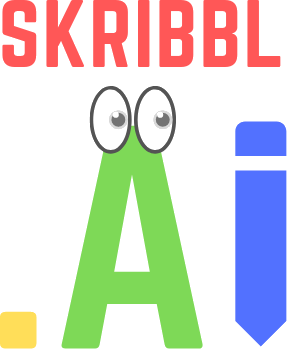
\includegraphics[width=0.25\textwidth]{images/skribbl_logo.png}
\caption{\label{fig:skribblLogo}Skribbl.AI Logo}
\end{wrapfigure}
Die Idee begann mit IQ gegen KI. Mit dem Einfall, was würde eigentlich passieren, wenn eine künstliche Intelligenz ein von einem Menschen gemaltes Bild  erkennen sollte? Neuronale Netzwerke erbringen beeindruckende Leistungen bei der Erkennung fotorealistischer Aufnahmen. Sie helfen sogar Pathologen bei der Erkennung von Krebszellen \parencite{ElizabethDougherty2018}. Was also würde also passieren, wenn wir eine künstliche Intelligenz mit den Kritzeleien einer Student*in konfrontieren?

 (Was ist das Projekt, wie ist es zustande gekommen, was ist das Ziel)
 \ref{fig:skribblLogo}

\subsection{Aufbau des Projektes}
    (Wir haben uns für agile, Scrum usw. entschieden)    1.2.1. Trello, Slack

\section{Grundlagen}
\subsection{Design}
\subsubsection{Findung Und SketchR}

Wissend, dass wir ein Spiel kreieren wollten, welches sowohl Bilderkennung durch ein neuronales Netzwerk garantiert als auch den Spielspaß für den Spieler, blieben wir bevor weitere Überlegungen angefangen werden konnten, direkt an Namen sowie Konzept des Projekts hängen.
Abgeleitet durch das englische Wort 'to scribble' mit ein paar wenigen Änderungen um den Namen für das deutsche Publikum besser aussprechbar zu machen, wurde 'Skribbl' geboren. Das Kürzel '.AI' hingegen war für uns als Team sehr offensichtlich. Nicht nur wäre es eine wundervolle URL, wenn jemand das Projekt veröffentlichen wollen würde, sondern sie zeigt ebenfalls die nahe Verbindung zum neuronalen Netzwerk.

Folgend kam die Entscheidung dahingehend, was für eine Art von Spiel wir erschaffen wollten. Eine Zeichnung sollte erkannt werden, aber die Möglichkeiten dies umzusetzen waren zu umfangreich und so mussten wir uns auf ein Konzept einigen. Eines, welches nicht zu \textit{viel} beinhaltete und den Rahmen nicht sprengen würde, allerdings auch nicht zu einfach ausfallen würde.

Letztendlich entschieden wir uns dafür erst einmal zu recherchieren, ob es nicht vielleicht bereits jemanden gab der ein ähnliches Konzept umgewandelt hat. Spiel oder nicht war dabei egal.
Dabei stießen wir auf zwei Seiten verschiedene Programme (SketchR und Quick, Draw! [Google]). Geholfen haben diese bei unserer Entscheidung in welche Richtung das Spiel sich entwickeln sollte definitiv. Nach einigen Diskussionen entschieden wir uns schließlich für ein Zeichen-Spiel mit integriertem Zeitfaktor, bei dem die Künstliche Intelligenz das Bild mit Hilfe eines Treppchen Systems (ist das gesuchte Wort wahrscheinlicher als alle anderen, somit ist es auf Platz 1), erkennen sollte.

\subsubsection{Mobile First}

Ein solches Projekt, mit Spiel-Charakter, wie man sie aus jedem App-Store kennt; kurze Level für ein Kurzweiliges Spielerlebnis machten eines schnell klar: Unsere Priorität lag auf Mobile-First.
Dabei musste der Touchscreen, die unterschiedlichen Bildschirmgrößen sowie Funktionen und Hürden der verschiedenen Browser und Betriebssysteme mit eingeplant werden. Dennoch war es für uns keine schwere Entscheidung den Desktop vorerst außen vor zu lassen und sicher zu stellen, dass unser Spiel wenigstens auf einem Smartphone spielbar ist.

\subsubsection{Accessibility}

Accessibility war ein Punkt, der zwar erst ein wenig später in unserem Projekt auftauchte, aber dennoch nicht von kleiner Bedeutung war. Mit dem sehr visuellen Thema des Zeichnens und der heutigen Einstellung zu Accessibility Themen, war uns schnell klar, dass wir unser Spiel so zugänglich wie möglich für alle Nutzer machen mussten.

Ein Styleguide (Styleguide anhängen?) wurde erstellt, in welchem jede Farbe und Schriftgröße so getestet wurde, dass sie den Werten der W3C Verordnung entspricht.
Gleichzeitig wurden noch andere Details beachtet, wie zum Beispiel welche Coding-Regeln einzuhalten waren.


\subsection{Frontend}
\subsection{Neuronales Netzwerk}
\subsubsection{Dataset}
\section{Anforderungen}
Genauere Productvision, Detailierter
\section{Umsetzung, Implementierung, Ausarbeitung}
\section{Spielbeschreibung, Ziel}
\section{Bewertung}
vgl. Anforderungen mit Ergebnis

\printbibliography
\end{document}
